\section{Architectural Views}

\subsection*{Process View}

	\begin{figure}[H]
	\centering
	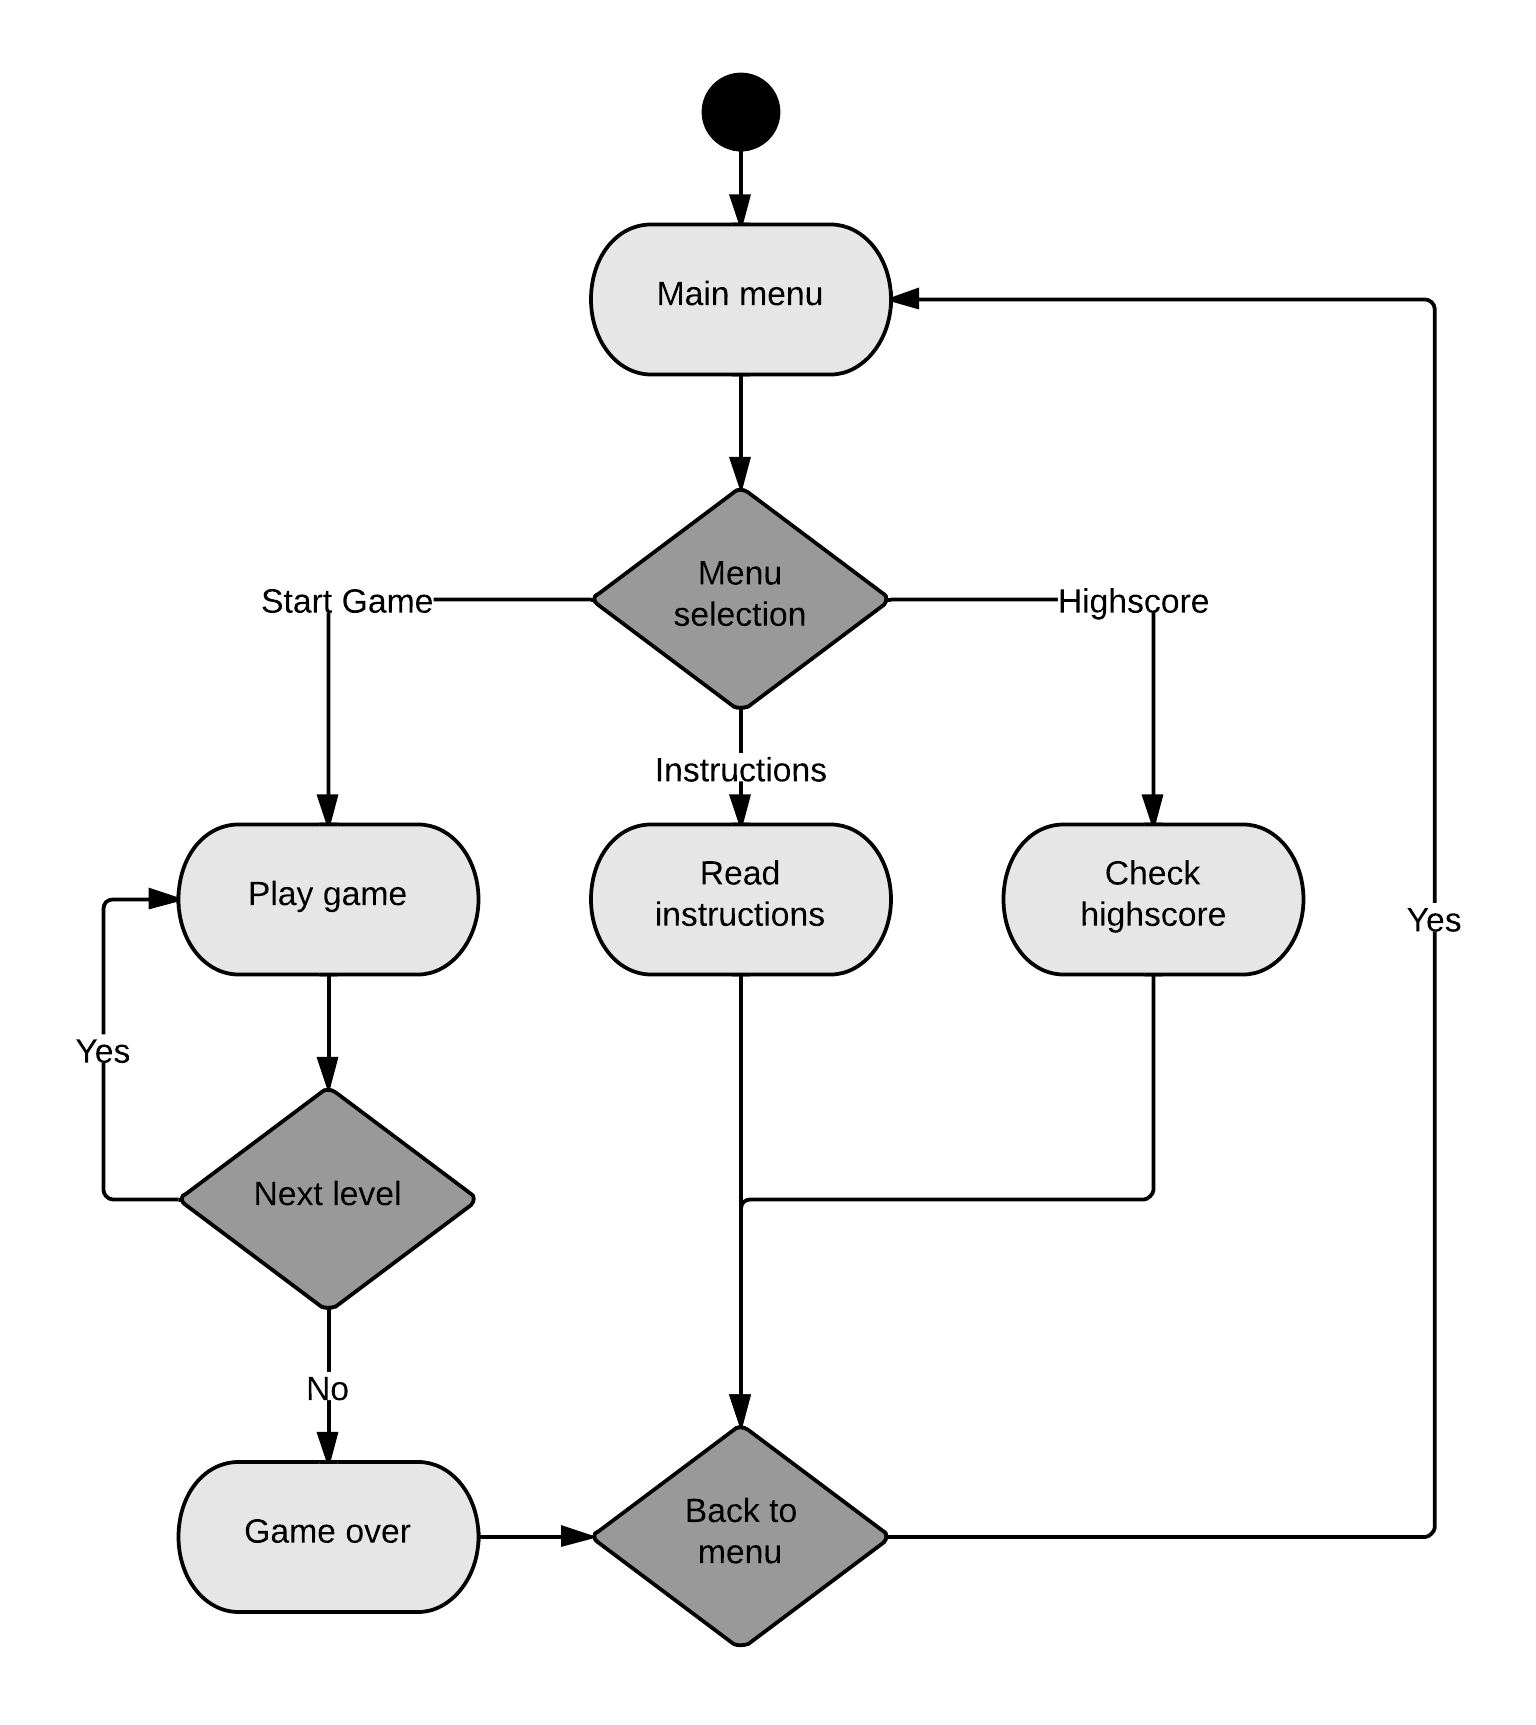
\includegraphics[width=\textwidth]{pictures/activity_diagram}
	\end{figure}

	The main menu screen is the entry point for the game. From there you can go to the "How to Play" screen, 
	to read about how the game works. You can go to the "Level Select" screen to start a new level, or load the 
	most recent level and continue playing from where you last left of. While playing you can exit the current 
	level and return to the main menu.

\subsection*{Logical View}

	The App object is the object where the game is started. It creates the game model and view objects 
	and starts the game. Because the game uses Backbone's Model-View-Presenter, all the game models 
	inherit Backbone Model. The Player object holds information about how much money the player got 
	available to them and the health. When the player's health reaches 0, the game is over. The Level 
	object holds general state information about the game. How long the player has been playing, the 
	current state of the game, etc. The Map object holds information about the game map which is going 
	to be drawn on the screen. The map has three collections, for the Powerplants, the Buildings and 
	the Powerlines. The Powerplants and Buidling objects placed on the game map. They inherit Entity, 
	which inherits Backbone Model. The Powerline object connects two entities and is used to create a
	network to distribute power.

	The objects inheriting Backbone View are Presenters. They listen to changes to the game models and 
	update the HTML objects with the state of the game. The Presenter objects also receive input events
	from the HTML and updates the models. The Screen object listens to the state of the game map, and
	updates the screen canvas. The HudMoney object listens to the player's money. The HudButtons object 
	receive input from the HTML and updates the game models. The HpBar object listens to changes to the 
	player's health. The Menu object receives input from the HTML and updates the game models.

	\begin{figure}[H]
	\begin{adjustwidth}{-50em}{-50em}
	\centering
	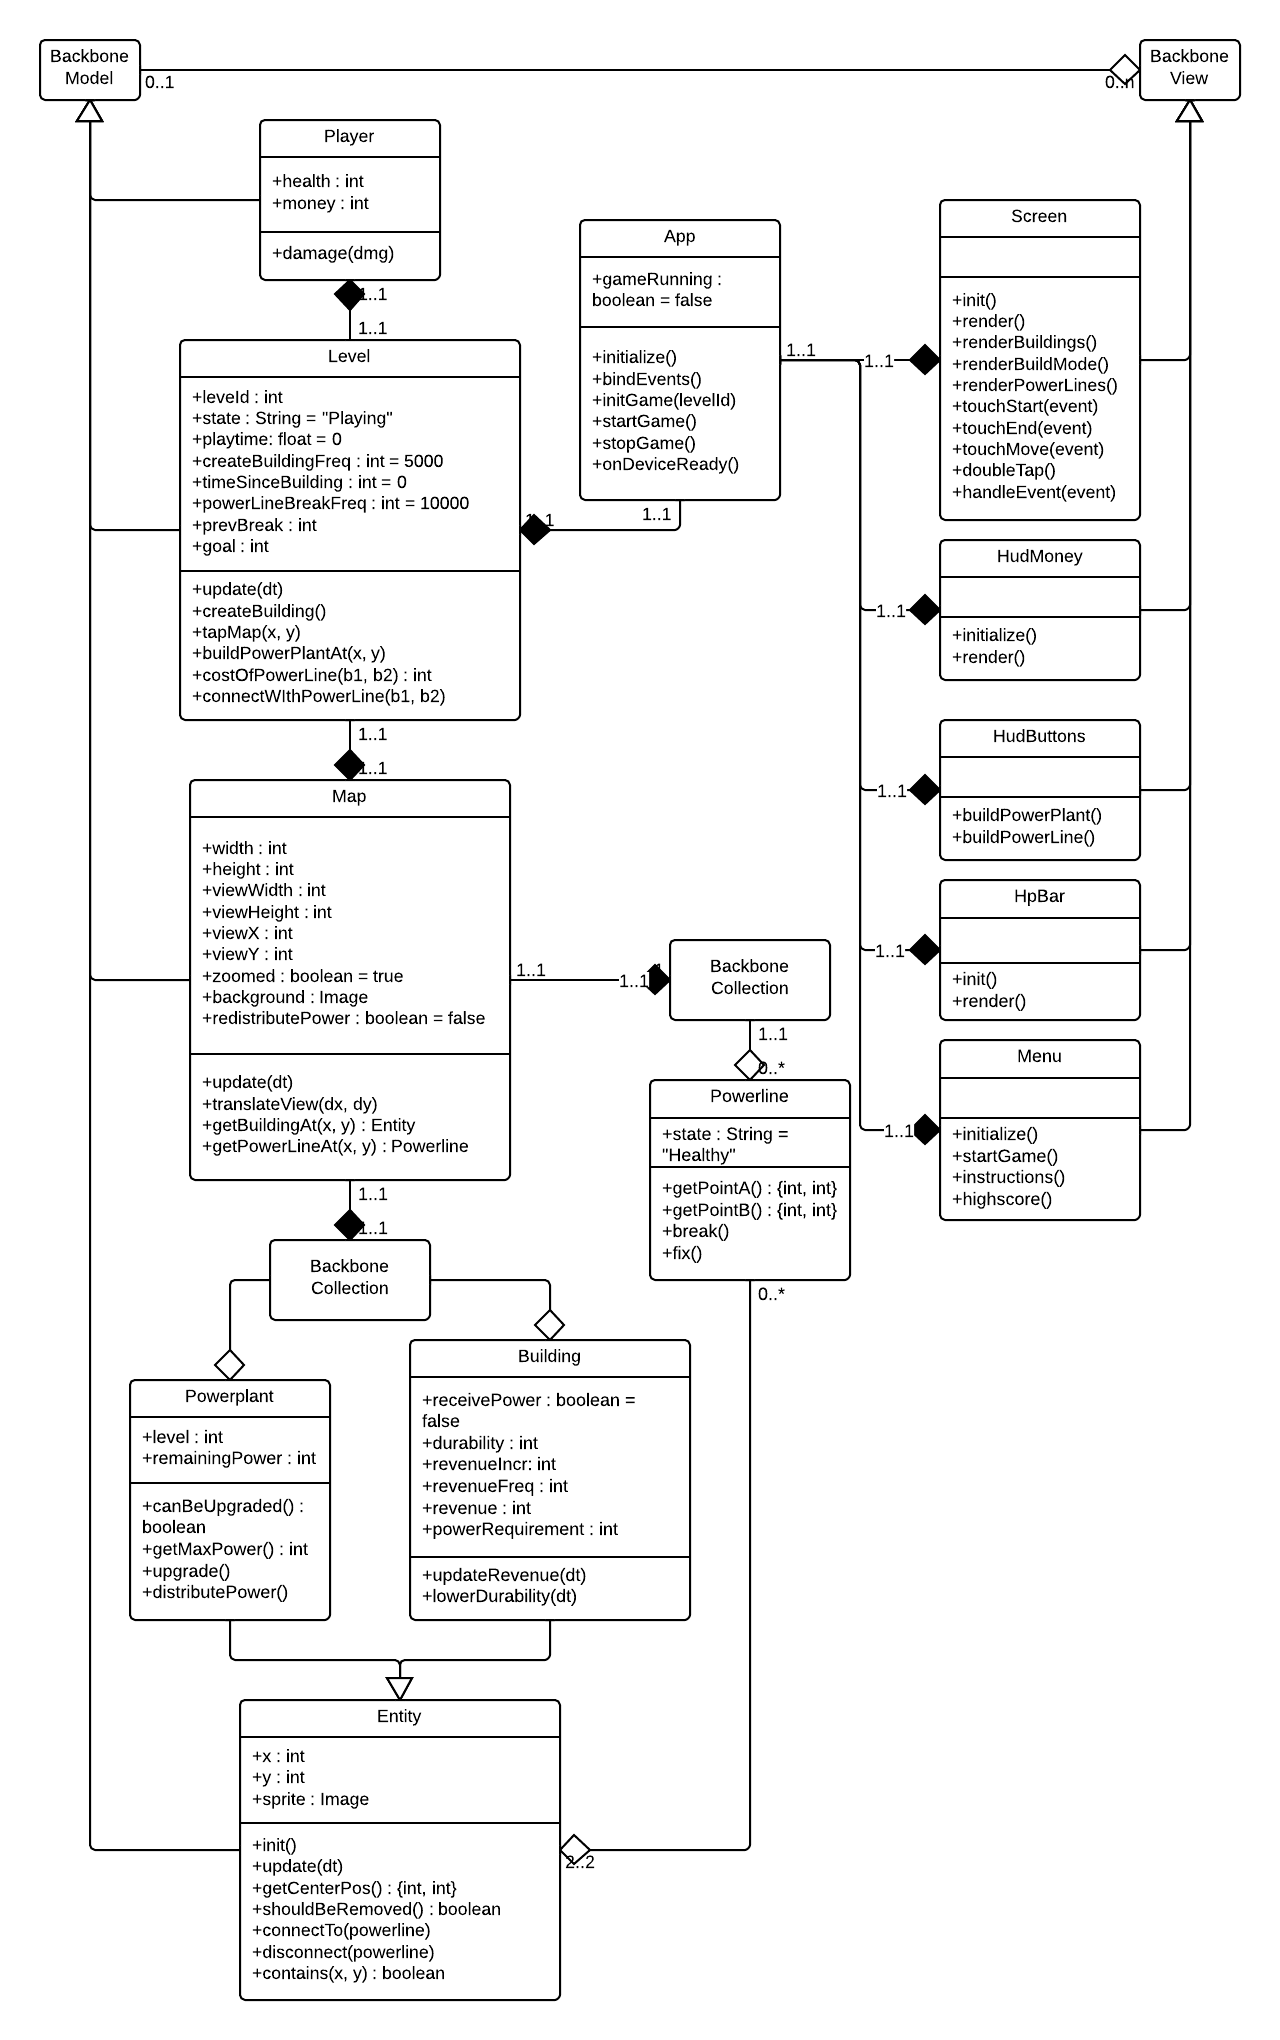
\includegraphics[scale=0.29]{pictures/class_diagram}
	\end{adjustwidth}
	\end{figure}

	\newpage

\subsection*{Physical View}

	We use Phonegap to handle the crossplatform deployment of our game. Phonegap creates a WebView for
	each native platform that we want to run our product on. The WebView then displays a webpage which
	runs our JavaScript code. Phonegap also allows us access to native platform functionality like
	storage, camera or the accelerometer without having to write the code for this functionality nativly
	for each platform.

	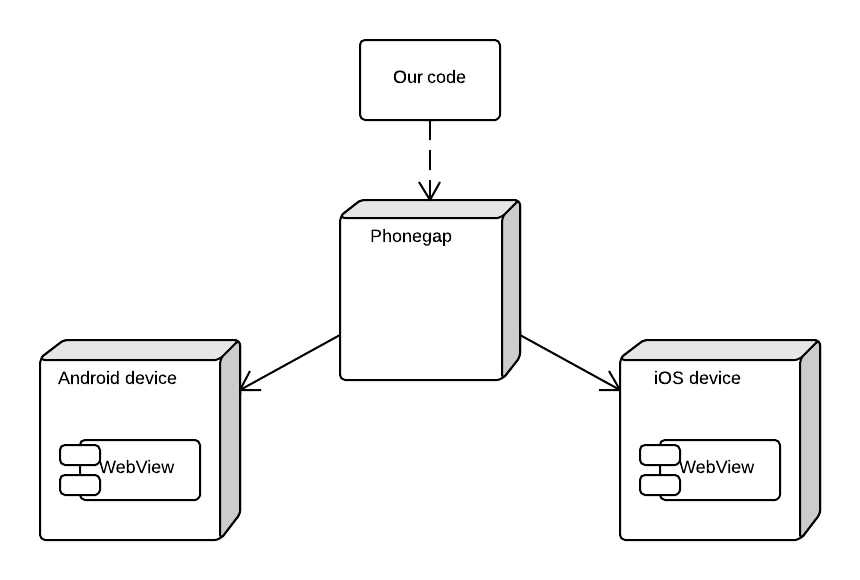
\includegraphics[width=\textwidth]{pictures/deployment_diagram}

\subsection*{Development View}

	The development view is separated into hierarchically into layers. The first layer is the game state 
	and logic layer. The Models store the current state of the game which gets updated by the game loop 
	and input from the player. The second layer decides how the game state is to be presented to the 
	player, this layer also receives user input from layer three which updates the game state. The third 
	layer is the HTML code which handles the layout of the user interface and sends user input to the
	second layer.

	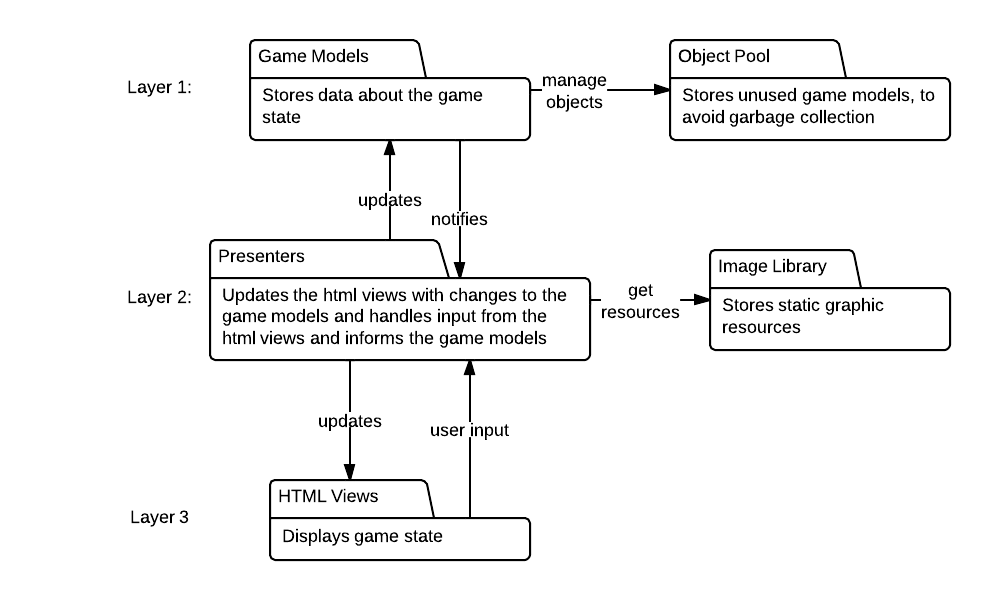
\includegraphics[width=\textwidth]{pictures/development_view}
